% Chapter 1

\newcommand{\VS}{\vspace{6pt}}
\newcommand{\vt}[1]{\vec{#1}}

\chapter{Dynamic Step} % Main chapter title

\label{Chapter1} % For referencing the chapter elsewhere, use \ref{Chapter1} 

%----------------------------------------------------------------------------------------

This modification is based on the constant step variant of the SVM-RFE algorithm, however, instead of using some constant number as the step in each iteration we calculate that number dynamically. The most straightforward way to do this is by using a percentage. Another possibility is to let the model score influence this percentage.

\section{Description and reasoning}

The percentage is a hyperparameter. It is used within every iteration to select a number of the first ranked features. A constant step has already been used in pract\-ice, but it is expected that this method will be significantly faster without effecting the accuracy performance, or even improving it.

The reasoning behind this is that when you have many features for which you only want to select a very small subset, the required amount of iterations will be of lineal complexity on the amount of features, however, by using a percentage, we get a logarithmic complexity.

Other similar modifications are also found in the literature, including using the square root of the remaining features \texttt{SQRT-RFE}, an entropy based function \texttt{E-RFE}, or \texttt{RFE-Annealing} which sets the step at $|\vt{s}| \frac{1}{i+1}$, thus, changing the percentage each iteration (\cite{ding_improving_2006}).

\iffalse
That is, the amount of features eliminated "$r$" at $j$-th iteration is the summation of the amount of features eliminated each iteration, i.e. $np^i$:

\begin{equation}\label{eq:dynamicStep1}
    r = \sum_{i = 1}^{j}{(np^i)} 
\end{equation}

It may be more interesting to see complexity as in the amount of iterations re\-quired to eliminate $r$ features, it can be derived from equation \ref{eq:dynamicStep1} as follows:

\begin{align*}
    r &= n \sum_{i = 1}^{j}{p^i} = n \sum_{i = 0}^{j-1}{(p^i)} - n + np^j \\
    \frac{r}{n} &= \frac{1-p^j}{1-p} - 1 + p^j \\
    \frac{r}{n} &= \frac{(1-p^j) - (1-p) + (1-p)p^j}{1-p}\\
    \frac{(1-p)r}{n} &= (1-p^j) - (1-p) + (p^j-p^{j+1})\\
    \frac{(1-p)r}{n} &= 1 -p^j -1 + p + p^j - p^{j+1}\\
    \frac{(1-p)r}{n} &= p - p^{j+1}\\
    - \frac{(1-p)r}{n} + p &= p^{j+1}\\
    \log_{p} \left( - \frac{(1-p)r - np}{n} \right) &= \log_{p} (p^{j+1})\\
    \log_{p} \left( - \frac{(1-p)r - np}{n} \right) &= j + 1\\
    \log_{1/p} \left( - \frac{n}{(1-p)r} + 1/p \right) &= j + 1\\
\end{align*}
\fi

We assume that, the bigger the step in each iteration, the worse the performance of the final selection. However, since we're selecting the worst variables first, se\-lect\-ing more of them at once shouldn't affect performance because they would have been selected anyway with height probability in the following iterations. The fewer the iterations remaining, the riskier it becomes selecting multiple variables at once, and thus a smaller step is beneficial.

\section{Pseudocode formalization}

\textbf{Definitions:}

\begin{itemize}
    \item $X_0 = [\vt{x_0}, \vt{x_1}, \dotsc, \vt{x_k}]^T$ list of observations.
    \item $\vt{y} = [y_1, y_2, \dotsc, y_k]^T$ list of labels.
\end{itemize}

\begin{algorithm}[H]
    \DontPrintSemicolon
      \KwInput{$p$ \tcp*{p = percentage, $0 \le p \le 1$}}
      \KwOutput{$\vt{r}$}
      \KwData{$X_0,\vt{y}$}
      $\vt{s} = [1,2, \dotsc, n]$ \tcp*{subset of surviving features}
      $\vt{r} = []$ \tcp*{feature ranked list} 
      \While{$|\vt{s}| > 0$}
        {
            \tcc*[h]{Restrict training examples to good feature indices}\\
            $X=X_0(:,\vt{s})$\VS

            \tcc*[h]{Train the classifier}\\
            $\vt{\alpha} = \texttt{SVM-train(} X, y \texttt{)}$\VS

            \tcc*[h]{Compute the weight vector of dimension length $|\vt{s}|$}\\
            $\vt{w} = \sum_k{\vt{\alpha_k} \vt{y_k} \vt{x_k}}$\VS

            \tcc*[h]{Compute the ranking criteria}\\
            $\vt{c} = [(w_i)^2 \text{ for all $i$}]$\VS

            \tcc*[h]{Compute $t$ based on the percentage}\\
            $t = p|\vt{s}|$\VS

            \tcc*[h]{Find the $t$ features with the smallest ranking criterion}\\
            $\vt{f} = \texttt{argsort}(\vt{c})(\ :t)$\VS

            \tcc*[h]{Update the feature ranking list}\\
            $\vt{r} = [\vt{s}(\vt{f}), ...\vt{r}]$\VS

            \tcc*[h]{Eliminate the features with the $t$ smallest ranking criterion}\\
            $\vt{s} = [[...\vt{s}(1:f_i - 1), ...\vt{s}(f_i + 1:|\vt{s}|)]$ for all $i]$
        }
    \caption{SVM-RFE with DynamicStep}
\end{algorithm}

\section{Results}

\subsection{Madelon Initial Analysis}

First, we're using the MADELON dataset. We've initially run some tests to find how the hyper-parameters (C and step) may influence it. 

The first test consists on simply doing a random feature selection and plotting the accuracy for the training and test splits. It is easy to see with figure \ref{fig:dynamicStep.madelon.base} that the classifier is not working too well with test data, even though good results appear on training data. This is probably due to overfitting. Reducing the amount of dimensions, even randomly, results on a slightly improved performance with a peak at 200 features.

\begin{figure}[h]
    \centering
    \begin{subfigure}[b]{0.4\linewidth}
        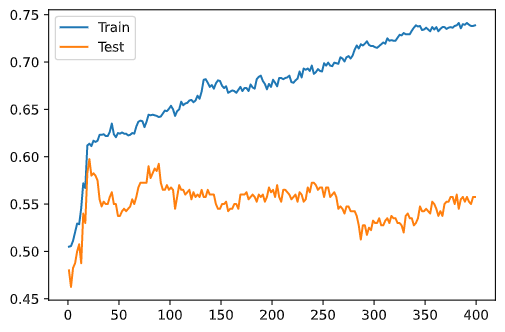
\includegraphics[width=\linewidth]{img/madelon-base-1.png}
        \subcaption*{$C=1$}
    \end{subfigure}
    \begin{subfigure}[b]{0.4\linewidth}
        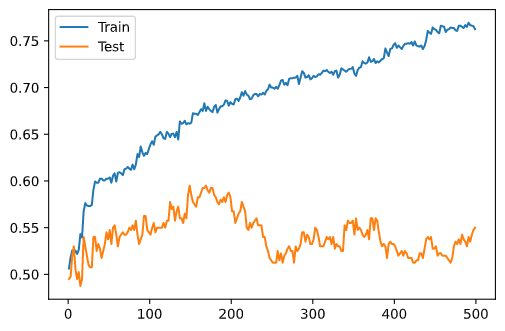
\includegraphics[width=\linewidth]{img/madelon-base-2.png}
        \subcaption*{$C=10^3$}
    \end{subfigure}
    \caption{Accuracy of an SVM classifier with a random feature selection with the Madelon dataset.}
    \label{fig:dynamicStep.madelon.base}
\end{figure}

We tested different values for the regularization parameter, from $10^0$ to $10^{12}$ in intervals of $1000$ times each, but there is no indication that this has any major effect.







